\chapter{General Project Context}

\section*{Preamble}

The telecommunications sector in Tunisia has experienced remarkable growth and technological advancement over the past decades, positioning itself as a cornerstone of the country's digital transformation. At the forefront of this evolution stands Tunisie Telecom, the national telecommunications operator, which manages an extensive network infrastructure spanning the entire territory. The complexity and scale of modern telecommunications networks necessitate sophisticated management systems to ensure optimal performance, reliability, and service quality for millions of subscribers across Tunisia.

This chapter presents the general context of the TelecomOps project, beginning with an in-depth examination of Tunisie Telecom as the host organization. We explore the fundamental challenges faced in mobile network site monitoring and management, analyze existing operational processes, and introduce our proposed solution. Finally, we outline the Scrum methodology adopted for project development, establishing the foundation for the technical and implementation phases that follow.

\section{Introduction}

The rapid expansion of mobile telecommunications infrastructure in Tunisia has created unprecedented operational challenges for network operators. With thousands of base transceiver stations distributed across diverse geographical locations, from urban centers to remote rural areas, the task of maintaining consistent network quality and availability has become increasingly complex. Each network site contains critical equipment requiring continuous monitoring, preventive maintenance, and rapid response to failures to ensure uninterrupted service delivery.

Traditional approaches to network infrastructure management, often relying on manual processes and fragmented systems, are no longer adequate to meet the demands of modern telecommunications operations. The need for integrated, real-time monitoring solutions has become paramount, driving the development of comprehensive management platforms that can provide visibility, control, and optimization capabilities across entire network infrastructures.

This project addresses these challenges through the development of TelecomOps, a web-based application specifically designed to modernize mobile network site management processes at Tunisie Telecom, enhancing operational efficiency and service reliability.

\section{Host Organization Presentation}

\subsection{Company Overview}

Tunisie Telecom, operating under the commercial name of the Office National des Télécommunications, stands as Tunisia's leading telecommunications operator since its establishment on April 17, 1995, becoming operational on January 1, 1996. As a public establishment attached to the Ministry of Communication Technologies, Tunisie Telecom has evolved to become the backbone of Tunisia's telecommunications infrastructure, serving millions of customers across the nation.

\begin{figure}[H]
    \centering
    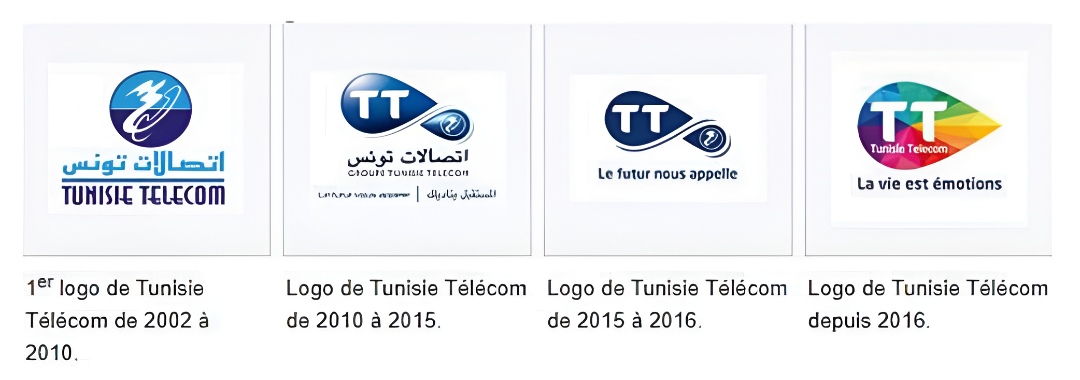
\includegraphics[width=0.8\columnwidth]{img/company/logos_update.png}
    \caption{Evolution of Tunisie Telecom Corporate Identity}
    \label{fig:tt_logos}
\end{figure}

The company's headquarters are strategically located in Tunis, from where it coordinates operations across 24 regional directions, maintaining over 80 customer service centers and leveraging a network of more than 13,000 private sales points throughout the country. This extensive organizational structure enables Tunisie Telecom to maintain close proximity to its customers while ensuring comprehensive territorial coverage.

\subsection{Service Portfolio}

Tunisie Telecom offers a comprehensive range of telecommunications services, positioning itself as a complete solutions provider for both individual and corporate customers:

\textbf{Fixed Line Services:} Traditional telephony services complemented by high-speed internet access through ADSL and fiber optic technologies, ensuring reliable connectivity for residential and business customers.

\textbf{Mobile Services:} Comprehensive mobile telecommunications offerings for individual consumers and enterprises, incorporating cutting-edge technologies including 3G, 4G, and 5G networks to deliver superior voice and data services.

\textbf{Internet Services:} High-speed internet access solutions for individuals, businesses, and public institutions, leveraging both fixed and mobile technologies to provide flexible connectivity options.

\textbf{Professional Services:} Specialized telecommunications solutions tailored to enterprise needs, including private network management, unified communication services, and customized infrastructure solutions.

\subsection{Organizational Structure}

The organizational architecture of Tunisie Telecom reflects its national scope and operational complexity. Under the leadership of a President and Chief Executive Officer, the company operates through multiple specialized directions coordinating various aspects of telecommunications operations.

\begin{figure}[H]
    \centering
    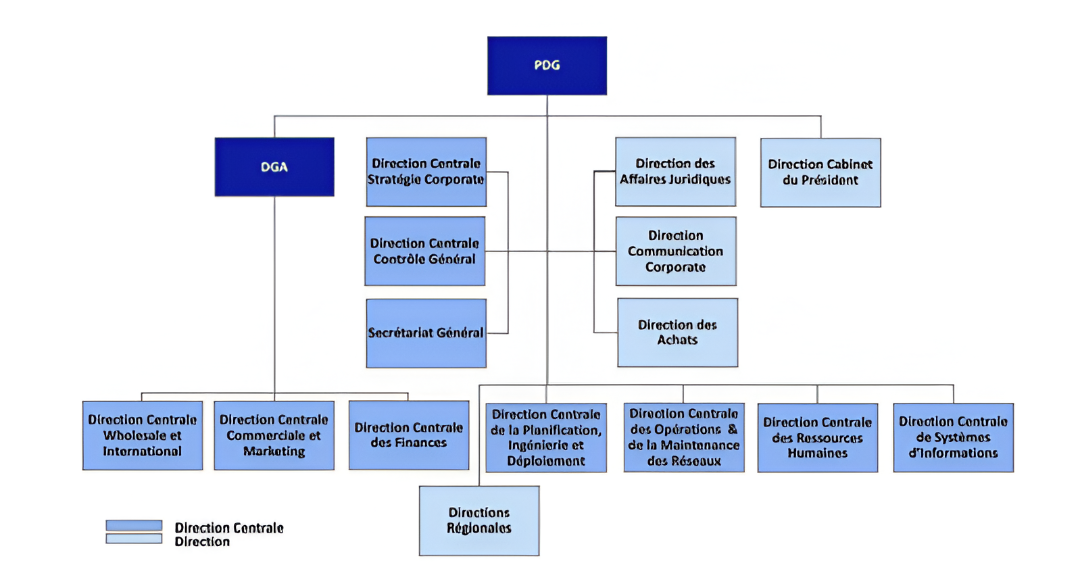
\includegraphics[width=0.9\columnwidth]{img/company/telecom_organigramme.png}
    \caption{Tunisie Telecom Organizational Structure}
    \label{fig:tt_organigramme}
\end{figure}

The structure encompasses specialized departments for network operations, customer service, technical infrastructure, human resources, finance, and strategic planning. This comprehensive organizational approach ensures effective coordination across all operational domains while maintaining focus on core telecommunications services.

\subsection{Workforce and Market Position}

Tunisie Telecom employs over 8,000 professionals across various technical and administrative functions, representing a significant concentration of telecommunications expertise within Tunisia. This substantial workforce enables the company to maintain its position as the country's telecommunications leader while continuously expanding and upgrading its infrastructure capabilities.

The company's market position is reinforced by its extensive infrastructure investments, technological innovation initiatives, and commitment to providing universal telecommunications access across all regions of Tunisia, including remote and underserved areas.

\section{Mobile Network Site Monitoring Problem Statement}

\subsection{Infrastructure Complexity Challenges}

The modern telecommunications landscape presents significant operational challenges for network operators managing large-scale infrastructure deployments. Tunisie Telecom's network comprises thousands of mobile sites distributed across Tunisia's diverse geographical terrain, each containing sophisticated equipment requiring continuous monitoring and maintenance.

These sites encompass multiple technology generations from 2G through 5G, each with distinct operational requirements and performance parameters. The heterogeneous nature of this infrastructure creates complexity in monitoring, maintenance scheduling, and performance optimization, requiring comprehensive management approaches to ensure consistent service quality.

\subsection{Traditional Management Limitations}

Current operational processes at Tunisie Telecom, like many telecommunications operators, rely heavily on manual procedures and disconnected systems for network site management. These approaches present several critical limitations:

\textbf{Data Fragmentation:} Information regarding site status, equipment inventory, maintenance records, and performance metrics is distributed across multiple systems and formats, making comprehensive visibility challenging and potentially leading to inconsistent decision-making.

\textbf{Reactive Maintenance Approach:} Without integrated monitoring capabilities, maintenance activities often follow reactive patterns, responding to failures after they impact service quality rather than preventing issues through proactive intervention.

\textbf{Limited Real-time Visibility:} The absence of centralized monitoring platforms restricts real-time visibility into network health, equipment status, and emerging issues, potentially extending problem resolution times and impacting customer experience.

\textbf{Resource Allocation Inefficiencies:} Manual processes for intervention planning and technician assignment can result in suboptimal resource utilization and delayed response to critical issues.

\textbf{Documentation and Audit Challenges:} Maintaining comprehensive records of maintenance activities, equipment changes, and intervention outcomes becomes difficult without integrated documentation systems, impacting audit capabilities and continuous improvement initiatives.

\section{Existing System Analysis}

\subsection{Current Operational Workflow}

The existing mobile network site management processes at Tunisie Telecom primarily rely on traditional approaches that have evolved over years of operational experience. These processes encompass several key areas:

\textbf{Site Information Management:} Basic site data, including location coordinates, equipment inventories, and configuration details, is maintained through spreadsheet applications and local databases. While functional, this approach creates data silos and synchronization challenges across different operational teams.

\textbf{Fault Detection and Reporting:} Network issues are typically identified through customer complaints, routine inspections, or automated alarm systems. However, the correlation and prioritization of these inputs require manual analysis, potentially leading to delays in critical issue identification.

\textbf{Maintenance Scheduling:} Preventive maintenance activities follow predetermined schedules based on equipment manufacturer recommendations and historical experience. The coordination of these activities relies on manual planning processes that may not optimally account for real-time operational conditions or resource availability.

\textbf{Intervention Management:} When issues arise, the assignment of technical personnel and coordination of repair activities follows established procedures, but lacks integrated tracking and progress monitoring capabilities that could enhance efficiency and accountability.

\subsection{Identified Limitations}

Through detailed analysis of current operations, several critical limitations have been identified:

\textbf{Scalability Constraints:} As the network continues to expand and technology complexity increases, manual processes become increasingly difficult to scale effectively, potentially impacting operational efficiency and service quality.

\textbf{Data Accuracy and Consistency:} The reliance on manual data entry and multiple disconnected systems creates risks of data inconsistency and accuracy issues, which can impact decision-making and operational planning.

\textbf{Performance Monitoring Gaps:} Limited integration between monitoring systems and operational processes restricts the ability to proactively identify performance trends and potential issues before they impact customers.

\textbf{Resource Optimization Opportunities:} Without comprehensive visibility into resource utilization patterns and intervention effectiveness, opportunities for optimization may be missed, impacting overall operational efficiency.

\section{Proposed Solution}

\subsection{TelecomOps Application Overview}

To address the identified challenges and limitations, we propose the development of TelecomOps, a comprehensive web-based application designed specifically for mobile network site management, operation, maintenance, and auditing. This solution leverages modern web technologies to provide an integrated platform that centralizes all aspects of network site management while providing the flexibility and scalability required for large-scale telecommunications operations.

TelecomOps is architected to serve as a centralized hub for all network site-related activities, providing different interfaces and capabilities tailored to various user roles within the organization. The application integrates site management, equipment tracking, fault monitoring, intervention planning, and performance analysis into a cohesive platform that enhances visibility and control across the entire network infrastructure.

\subsection{Core Functional Capabilities}

\textbf{Comprehensive Site Management:} The application provides complete lifecycle management for network sites, including detailed site profiles, location management, technology configuration tracking, and equipment inventory management for 2G, 3G, 4G, and 5G installations.

\textbf{Equipment Monitoring and Tracking:} Detailed equipment inventories with tracking capabilities for installation dates, maintenance schedules, performance metrics, and replacement planning, ensuring optimal equipment lifecycle management.

\textbf{Intelligent Alert System:} Real-time alert generation and management capabilities that prioritize issues based on severity levels, impact analysis, and predefined escalation procedures, enabling rapid response to critical situations.

\textbf{Breakdown Management:} Comprehensive fault tracking and resolution workflows that document issue identification, diagnosis procedures, resolution activities, and outcome analysis to support continuous improvement initiatives.

\textbf{Intervention Planning and Tracking:} Advanced scheduling and coordination capabilities for both preventive and corrective maintenance activities, including resource allocation, progress tracking, and outcome documentation.

\textbf{Role-Based Access Control:} Sophisticated user management with differentiated access levels for administrators, network engineers, field technicians, and operational managers, ensuring appropriate information access and functional capabilities for each role.

\subsection{Technical Architecture}

The TelecomOps solution is built on a modern, scalable technical architecture that ensures performance, reliability, and maintainability:

\textbf{Frontend Technology:} Next.js framework with TypeScript provides a responsive, high-performance user interface that adapts to various devices and screen sizes while ensuring type safety and development efficiency.

\textbf{Backend Services:} Supabase provides a robust backend-as-a-service platform with PostgreSQL database management, real-time capabilities, and integrated authentication services, ensuring scalable data management and secure access control.

\textbf{Database Design:} A comprehensive relational database schema optimized for telecommunications operations, incorporating entities for sites, equipment, interventions, alerts, user profiles, and audit trails.

\begin{figure}[H]
    \centering
    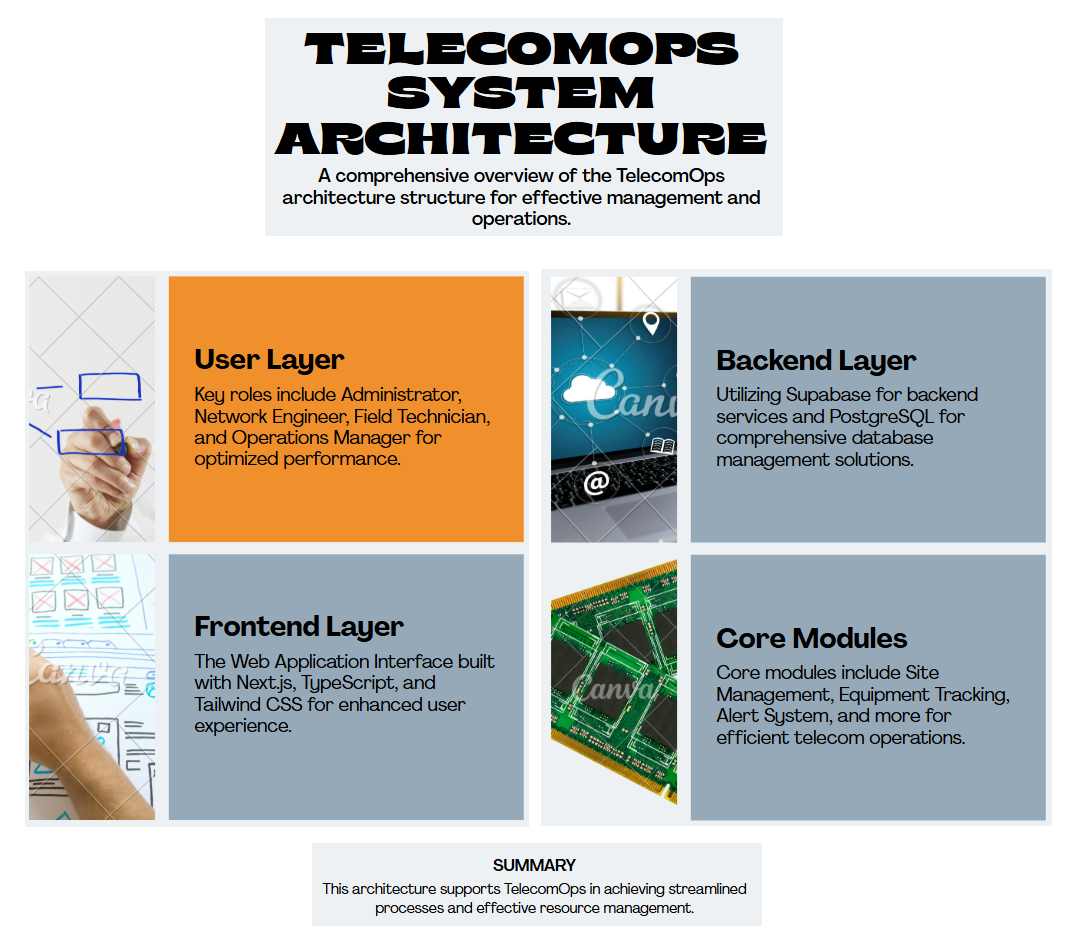
\includegraphics[width=0.9\columnwidth]{img/TELECOMOPS SYSTEM ARCHITECTURE.png}
    \caption{TelecomOps Technical Architecture Overview}
    \label{fig:architecture}
\end{figure}

\subsection{Expected Benefits and Outcomes}

The implementation of TelecomOps is expected to deliver significant operational benefits:

\textbf{Enhanced Operational Efficiency:} Streamlined processes and automated workflows will reduce manual effort and improve response times for critical issues.

\textbf{Improved Network Reliability:} Proactive monitoring and preventive maintenance capabilities will reduce unplanned downtime and enhance overall network performance.

\textbf{Better Resource Utilization:} Optimized scheduling and resource allocation will improve technician productivity and reduce operational costs.

\textbf{Enhanced Decision Making:} Comprehensive reporting and analytics capabilities will provide insights for strategic planning and operational optimization.

\textbf{Regulatory Compliance:} Integrated documentation and audit trails will support regulatory compliance requirements and internal quality assurance processes.

\section{Project Management Methodology Study}

The organization, management, and supervision of resources, tasks, and processes are essential to achieve specific objectives within a determined timeframe. Different project management methods exist, each adapting to specific projects, environments, and requirements.

\subsection{Main Agile Methodologies}

\subsubsection{Scrum}

The Agile Scrum method is one of the most appreciated approaches. Its structure is based on sprints (2 to 4-week iterations), which rely on specific roles such as Product Owner, Scrum Master, and development team. Each sprint must deliver a functional version of the product, with work subdivided into sections called "user stories."

\begin{figure}[H]
    \centering
    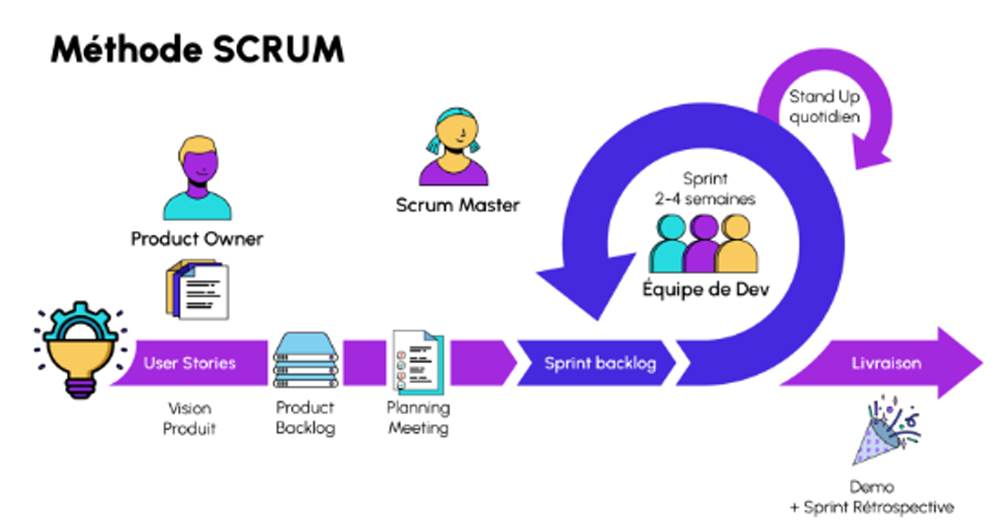
\includegraphics[width=0.9\columnwidth]{img/architecture/Scrum.png}
    \caption{Scrum Development Process}
    \label{fig:scrum_process}
\end{figure}

\subsubsection{Kanban}

Kanban is a visual task management method. Kanban boards are used to track tasks through different completion stages (for example "To Do", "In Progress", "Done"). Unlike Scrum, Kanban does not require fixed sprints and operates continuously.

\begin{figure}[H]
    \centering
    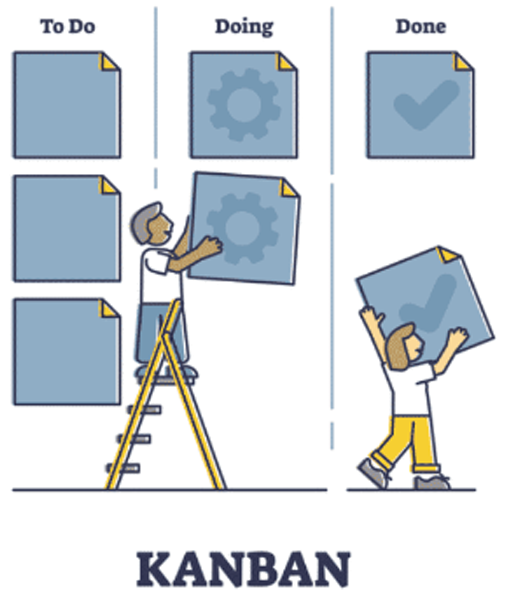
\includegraphics[width=0.6\columnwidth]{img/architecture/kanban.png}
    \caption{Kanban Process Flow}
    \label{fig:kanban_process}
\end{figure}

\subsubsection{Extreme Programming (XP)}

Extreme Programming (XP) emphasizes code quality and continuous programming improvement. It encourages the use of techniques such as pair programming, automated testing, and short development sessions.

\begin{figure}[H]
    \centering
    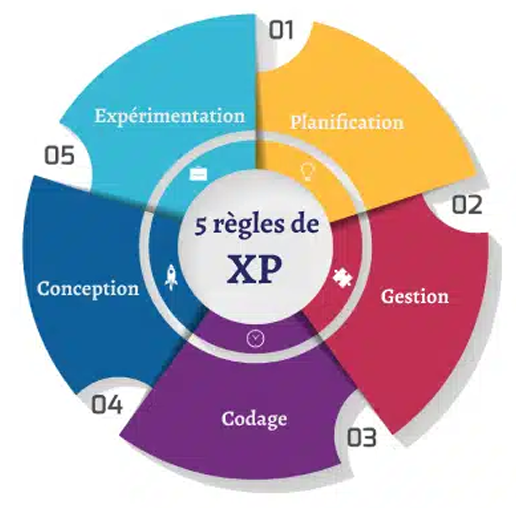
\includegraphics[width=0.6\columnwidth]{img/architecture/Extreme Programming.png}
    \caption{Extreme Programming (XP) Development Process}
    \label{fig:xp_process}
\end{figure}

\subsection{Chosen Method: Scrum}

Due to its characteristics, the Scrum method has been chosen to manage this project, making it particularly suitable for dynamic and complex environments. Scrum offers an iterative and flexible environment that facilitates efficient management of constantly evolving priorities, continuous value production, and close involvement of stakeholders.

Through the use of backlogs, adopting this methodology also provides a more precise vision of tasks to be performed and those in progress.

\subsubsection{Role Definitions}

An agile project presents different responsibilities and tasks from a sequential project, as it emphasizes project ownership by each team member while preserving collaboration.

The team consists of three main actors:

\textbf{Product Owner:} Represents the end users (or clients) of the project. Main responsibilities include:
\begin{itemize}
    \item Determining functional characteristics
    \item Analyzing features to improve or enhance
    \item Reviewing developed features
\end{itemize}

\textbf{Scrum Master:} Their role in the project team is to ensure compliance with Scrum principles and values. Additionally, they establish communication between team members to improve productivity and expertise.

\textbf{Development Team:} Works technically on user stories, evaluates their complexity, and ensures that technical requirements needed for product delivery are met, reporting any problems or obstacles in the process.

\subsubsection{Scrum Artifacts}

\textbf{Product Backlog:} A list of suggested activities indicating those to be performed during the project. Each operation is associated with various criteria desired by the client. Each item is listed according to priority given by the client.

\textbf{Sprint Backlog:} Represents tasks that must be completed within a specific timeframe, meaning each developer must respect the required deadline to accomplish each task. Each sprint is based on objectives established at its beginning.

\begin{table}[H]
\centering
\begin{tabular}{|l|p{10cm}|}
\hline
\textbf{Scrum Element} & \textbf{Description} \\
\hline
Sprint Duration & 2-4 weeks fixed iterations \\
\hline
Daily Scrum & 15-minute daily synchronization meetings \\
\hline
Sprint Planning & Meeting to define sprint goals and select backlog items \\
\hline
Sprint Review & Demonstration of completed work to stakeholders \\
\hline
Sprint Retrospective & Team reflection on process improvements \\
\hline
\end{tabular}
\caption{Scrum Framework Elements}
\label{tab:scrum_elements}
\end{table}

\subsection{Sprint Organization Structure}

The TelecomOps development process is structured across six distinct sprints, each addressing specific functional domains:

\textbf{Sprint 1:} Foundation development including authentication systems, user management, and basic site management capabilities, establishing the core platform infrastructure.

\textbf{Sprint 2:} Equipment inventory management and tracking systems, providing comprehensive equipment lifecycle management capabilities.

\textbf{Sprint 3:} Breakdown management and intervention planning modules, addressing fault detection, reporting, and resolution workflows.

\textbf{Sprint 4:} Alert system implementation and energy monitoring capabilities, enabling real-time network health monitoring and proactive issue identification.

\textbf{Sprint 5:} Reporting and analytics functionality, providing comprehensive dashboards and data analysis capabilities for operational insights.

\textbf{Sprint 6:} Deployment preparation, testing coordination, and continuous integration pipeline establishment, ensuring production readiness and maintainability.

\subsection{Quality Assurance and Testing}

Throughout the Scrum process, quality assurance activities are integrated into each sprint cycle. This includes unit testing development, integration testing protocols, user acceptance testing coordination, and performance validation procedures. The iterative nature of Scrum enables continuous quality improvement and early identification of potential issues.

Testing activities encompass functional validation, security assessment, performance evaluation, and user experience verification, ensuring that each delivered increment meets both technical specifications and operational requirements.

\section*{Conclusion}

This chapter has established the comprehensive context for the TelecomOps project, highlighting the critical importance of modern network management solutions in Tunisia's telecommunications landscape. Through detailed analysis of Tunisie Telecom as the host organization, we have identified the specific operational challenges and limitations that drive the need for integrated management platforms.

The proposed TelecomOps solution addresses these challenges through a comprehensive, technology-forward approach that leverages modern web development technologies and proven development methodologies. The adoption of Scrum ensures structured, iterative development that incorporates stakeholder feedback while maintaining focus on delivering practical, operational value.

The foundation established in this chapter provides the groundwork for the detailed planning and architectural phases that follow, setting clear expectations for the technical implementation and expected outcomes of the TelecomOps project.